% !TEX program = xelatex
\documentclass[12pt,a4paper]{ctexart}

% ── 页面与排版 ──────────────────────────────────────
\usepackage[top=2.5cm,bottom=2.5cm,left=2.5cm,right=2.5cm]{geometry}
\usepackage{setspace}
\onehalfspacing

% ── 数学 ────────────────────────────────────────────
\usepackage{amsmath,amssymb}

% ── 图表 ────────────────────────────────────────────
\usepackage{graphicx}
\graphicspath{{figures/}}
\usepackage{float}
\usepackage{booktabs}
\usepackage{multirow}
\usepackage{makecell}
\usepackage{longtable}
\usepackage{caption}
\usepackage{subcaption}

% ── 代码 ────────────────────────────────────────────
\usepackage{listings}
\usepackage{xcolor}
\lstset{
  basicstyle=\small\ttfamily,
  keywordstyle=\color{blue}\bfseries,
  commentstyle=\color{gray},
  stringstyle=\color{red!70!black},
  numbers=left, numberstyle=\tiny\color{gray},
  frame=single, framesep=3pt,
  breaklines=true, breakatwhitespace=true,
  tabsize=4,
  showstringspaces=false,
  captionpos=b,
  xleftmargin=2em,
  aboveskip=1em, belowskip=1em,
}

% ── 超链接 ──────────────────────────────────────────
\usepackage{hyperref}
\hypersetup{
  colorlinks=true,
  linkcolor=black,
  citecolor=blue,
  urlcolor=blue!70!black,
  bookmarksnumbered=true,
}

% ── 页眉页脚 ────────────────────────────────────────
\usepackage{fancyhdr}
\pagestyle{fancy}
\fancyhf{}
\fancyhead[L]{\small 数据库引论\,——\,项目报告}
\fancyhead[R]{\small \leftmark}
\fancyfoot[C]{\thepage}
\renewcommand{\headrulewidth}{0.4pt}

% ── 其他 ────────────────────────────────────────────
\usepackage{enumitem}
\setlist{nosep,leftmargin=2em}
\usepackage{tikz}
\usetikzlibrary{shapes.geometric,arrows.meta,positioning,fit,calc}

% ── 自定义命令 ──────────────────────────────────────
\newcommand{\code}[1]{\texttt{#1}}
\newcommand{\api}[1]{\texttt{#1}}

% ════════════════════════════════════════════════════
\begin{document}

% ── 封面 ────────────────────────────────────────────
\begin{titlepage}
\centering
\vspace*{3cm}
{\Huge\bfseries 学术论文搜索与推荐系统\\[0.6em]
\Large Academic Paper Search \& Recommend System}

\vspace{2cm}
{\Large 数据库引论\,——\,项目报告}

\vspace{3cm}
\begin{tabular}{rl}
\textbf{课程名称：} & 数据库引论实验课 \\[0.5em]
\textbf{选题方向：} & 论文搜索与推荐 \\[0.5em]
\textbf{姓\qquad 名：} & 年骏杰 \\[0.5em]
\textbf{学\qquad 号：} & 24307140012 \\[0.5em]
\textbf{提交日期：} & 2026 年 6 月 1 日 \\
\end{tabular}

\vfill
\end{titlepage}

% ── 目录 ────────────────────────────────────────────
\newpage
\tableofcontents
\newpage

% ════════════════════════════════════════════════════
% 第一章：项目概述
% ════════════════════════════════════════════════════
\section{项目概述}

\subsection{项目背景}

随着学术论文数量的爆炸式增长，研究者在海量文献中高效检索并发现有价值的论文成为一项重要需求。传统的关键词匹配搜索仅能捕获字面重合，无法理解查询的语义意图。本项目面向数据库与数据管理领域，构建了一套融合\textbf{向量语义检索}、\textbf{基于Embedding质心的个性化推荐}、\textbf{可选精排}、\textbf{PDF全文提取与分块Embedding}以及\textbf{基于RAG的大语言模型学术问答}的全栈论文搜索与推荐系统。

\subsection{选题说明}

本项目选题为"\textbf{论文搜索与推荐}"：根据用户输入的自然语言查询，从论文库中语义搜索论文；根据用户的点击浏览历史，个性化推荐相关论文；同时集成LLM多轮对话，辅助用户理解论文内容。

\subsection{技术栈总览}

\begin{table}[H]
\centering
\caption{系统技术栈}
\label{tab:techstack}
\begin{tabular}{llll}
\toprule
\textbf{层级} & \textbf{技术} & \textbf{版本} & \textbf{说明} \\
\midrule
\multirow{4}{*}{前端 (界面层)}
  & Vue 3          & 3.4.21 & Composition API \\
  & Element Plus   & 2.6.3  & UI组件库 \\
  & Pinia          & 2.1.7  & 状态管理 \\
  & Vite           & 5.1.6  & 构建工具 \\
\midrule
\multirow{4}{*}{业务层}
  & FastAPI        & 0.114.0 & 异步Web框架 \\
  & SQLAlchemy     & 2.0.35  & ORM \\
  & PyJWT          & 2.8.0   & JWT认证 \\
  & Passlib+bcrypt & —       & 密码哈希 \\
\midrule
\multirow{4}{*}{算法层}
  & FastAPI        & 0.114.0 & 独立微服务 \\
  & ChromaDB       & —       & 向量数据库 \\
  & NumPy          & —       & 数值计算 \\
  & PyMuPDF (fitz) & 1.27    & PDF全文提取 \\
\midrule
\multirow{2}{*}{存储}
  & MySQL 8.0+     & —       & 关系型数据库 \\
  & ChromaDB       & —       & 向量索引持久化 \\
\midrule
\multirow{3}{*}{模型}
  & text-embedding-v4 & 1024维 & 语义向量化 \\
  & qwen-flash        & —      & LLM对话 \\
  & qwen3-rerank      & —      & 可选精排 \\
\bottomrule
\end{tabular}
\end{table}


% ════════════════════════════════════════════════════
% 第二章：系统架构设计
% ════════════════════════════════════════════════════
\section{系统架构设计}

\subsection{分层架构}

系统严格遵循课程要求的\textbf{三层分离架构}：界面层负责与用户交互，业务层处理逻辑与数据持久化，算法层专注核心搜索/推荐/对话算法。各层通过HTTP RESTful API通信，可独立部署与扩展。

\begin{figure}[H]
\centering
\begin{tikzpicture}[
    layer/.style={draw, rounded corners, minimum width=14cm, minimum height=1.8cm, align=center, font=\small},
    comp/.style={draw, rounded corners=3pt, minimum width=2.5cm, minimum height=0.8cm, align=center, font=\footnotesize},
    db/.style={draw, cylinder, shape border rotate=90, aspect=0.25, minimum width=1.8cm, minimum height=1cm, font=\footnotesize},
    arr/.style={-{Stealth[length=5pt]}, thick},
    note/.style={font=\footnotesize\itshape, text=gray},
]

% 界面层
\node[layer, fill=blue!8] (ui) at (0, 6) {};
\node[font=\small\bfseries, anchor=west] at (-6.8, 6.5) {界面层};
\node[note, anchor=east] at (6.8, 6.5) {Vue 3 + Element Plus\quad :5173};
\node[comp, fill=blue!15] (search_ui) at (-4, 5.8) {论文搜索};
\node[comp, fill=blue!15] (rec_ui)    at (-1, 5.8) {论文推荐};
\node[comp, fill=blue!15] (chat_ui)   at (2, 5.8)  {AI对话};
\node[comp, fill=blue!15] (user_ui)   at (5, 5.8)  {用户管理};

% 业务层
\node[layer, fill=green!8] (biz) at (0, 3.5) {};
\node[font=\small\bfseries, anchor=west] at (-6.8, 4.1) {业务层};
\node[note, anchor=east] at (6.8, 4.1) {FastAPI + MySQL\quad :8000};
\node[comp, fill=green!15] (auth)   at (-4.5, 3.3) {JWT认证};
\node[comp, fill=green!15] (crud)   at (-1.5, 3.3) {论文CRUD};
\node[comp, fill=green!15] (proxy)  at (1.5, 3.3)  {搜索/推荐代理};
\node[comp, fill=green!15] (sse)    at (4.5, 3.3)  {SSE聊天转发};

% 算法层
\node[layer, fill=orange!8] (algo) at (0, 1) {};
\node[font=\small\bfseries, anchor=west] at (-6.8, 1.6) {算法层};
\node[note, anchor=east] at (6.8, 1.6) {FastAPI + ChromaDB\quad :8003};
\node[comp, fill=orange!15] (vec_search) at (-4, 0.8) {向量语义检索};
\node[comp, fill=orange!15] (centroid)   at (-0.5, 0.8) {质心推荐};
\node[comp, fill=orange!15] (rerank)     at (2.5, 0.8)  {Reranker};
\node[comp, fill=orange!15] (llm)        at (5, 0.8)    {LLM对话};

% 数据库
\node[db, fill=green!10]  (mysql)  at (-4, -1.2) {MySQL};
\node[db, fill=orange!10] (chroma) at (0, -1.2) {ChromaDB};
\node[db, fill=red!10]    (dash)   at (4, -1.2) {DashScope};

% 箭头
\draw[arr] (ui) -- node[right, note]{/api/* 代理} (biz);
\draw[arr] (biz) -- node[right, note]{HTTP / SSE} (algo);
\draw[arr] (auth.south) -- ++(0, -1.2) -- (mysql.north);
\draw[arr] (crud.south) -- ++(0, -0.6) -- ++(-2.5,0) -- (mysql.north);
\draw[arr] (vec_search.south) -- ++(0, -0.5) -- ++(4,0) -- (chroma.north);
\draw[arr] (centroid.south) -- (chroma.north);
\draw[arr] (llm.south) -- ++(0, -0.5) -- ++(0,0) -- (dash.north);

\end{tikzpicture}
\caption{系统三层架构图}
\label{fig:arch}
\end{figure}

\subsection{数据流设计}

系统的三条核心数据流如下：

\begin{enumerate}
\item \textbf{搜索流程}：用户输入查询 $\to$ 业务层记录搜索历史至MySQL $\to$ 转发至算法层 $\to$ 查询文本经\code{text-embedding-v4}向量化 $\to$ ChromaDB ANN检索 $\to$ 可选Reranker精排 $\to$ 返回\code{paper\_id + score} $\to$ 业务层从MySQL补全论文元数据 $\to$ 分页返回前端。

\item \textbf{推荐流程}：用户浏览论文时前端调用\api{/click}接口记录点击 $\to$ 请求推荐时业务层获取用户最近50条点击 $\to$ 算法层从ChromaDB获取已点击论文的Embedding $\to$ 计算质心向量 $\to$ ChromaDB近邻搜索 $\to$ 过滤已读 $\to$ 返回Top-K推荐。

\item \textbf{对话流程（三种模式）}：
  \begin{itemize}
  \item \textbf{论文问答模式}：论文详情页提问 $\to$ 业务层调用算法层\api{/search-chunks}按\code{paper\_id}检索该论文全文分块 $\to$ 注入论文元信息与全文片段 $\to$ LLM基于全文内容回答。
  \item \textbf{RAG全库模式}：AI对话页提问 $\to$ 业务层调用\api{/search-chunks}全库检索最相关分块 $\to$ 按论文聚合并注入上下文 $\to$ LLM回答并附带参考论文列表 $\to$ 前端显示可点击的引用标签。
  \item \textbf{纯对话模式}：注入用户最近5篇已读论文摘要 $\to$ 转发至算法层 $\to$ SSE流式返回。
  \end{itemize}

\item \textbf{全文索引流程}：PDF全文经PyMuPDF提取 $\to$ 按约800词/块分块（100词重叠）$\to$ 批量调用算法层\api{/index-chunks} $\to$ Embedding后存入ChromaDB \code{paper\_chunks} collection。
\end{enumerate}

\textbf{降级机制}：当算法层不可用时，搜索自动降级为MySQL \code{LIKE}模糊匹配，保障系统基本可用性。


% ════════════════════════════════════════════════════
% 第三章：数据库设计
% ════════════════════════════════════════════════════
\section{数据库设计}

\subsection{ER图}

系统包含4张核心表，通过外键关联形成完整的数据模型。

\begin{figure}[H]
\centering
\resizebox{0.96\textwidth}{!}{%
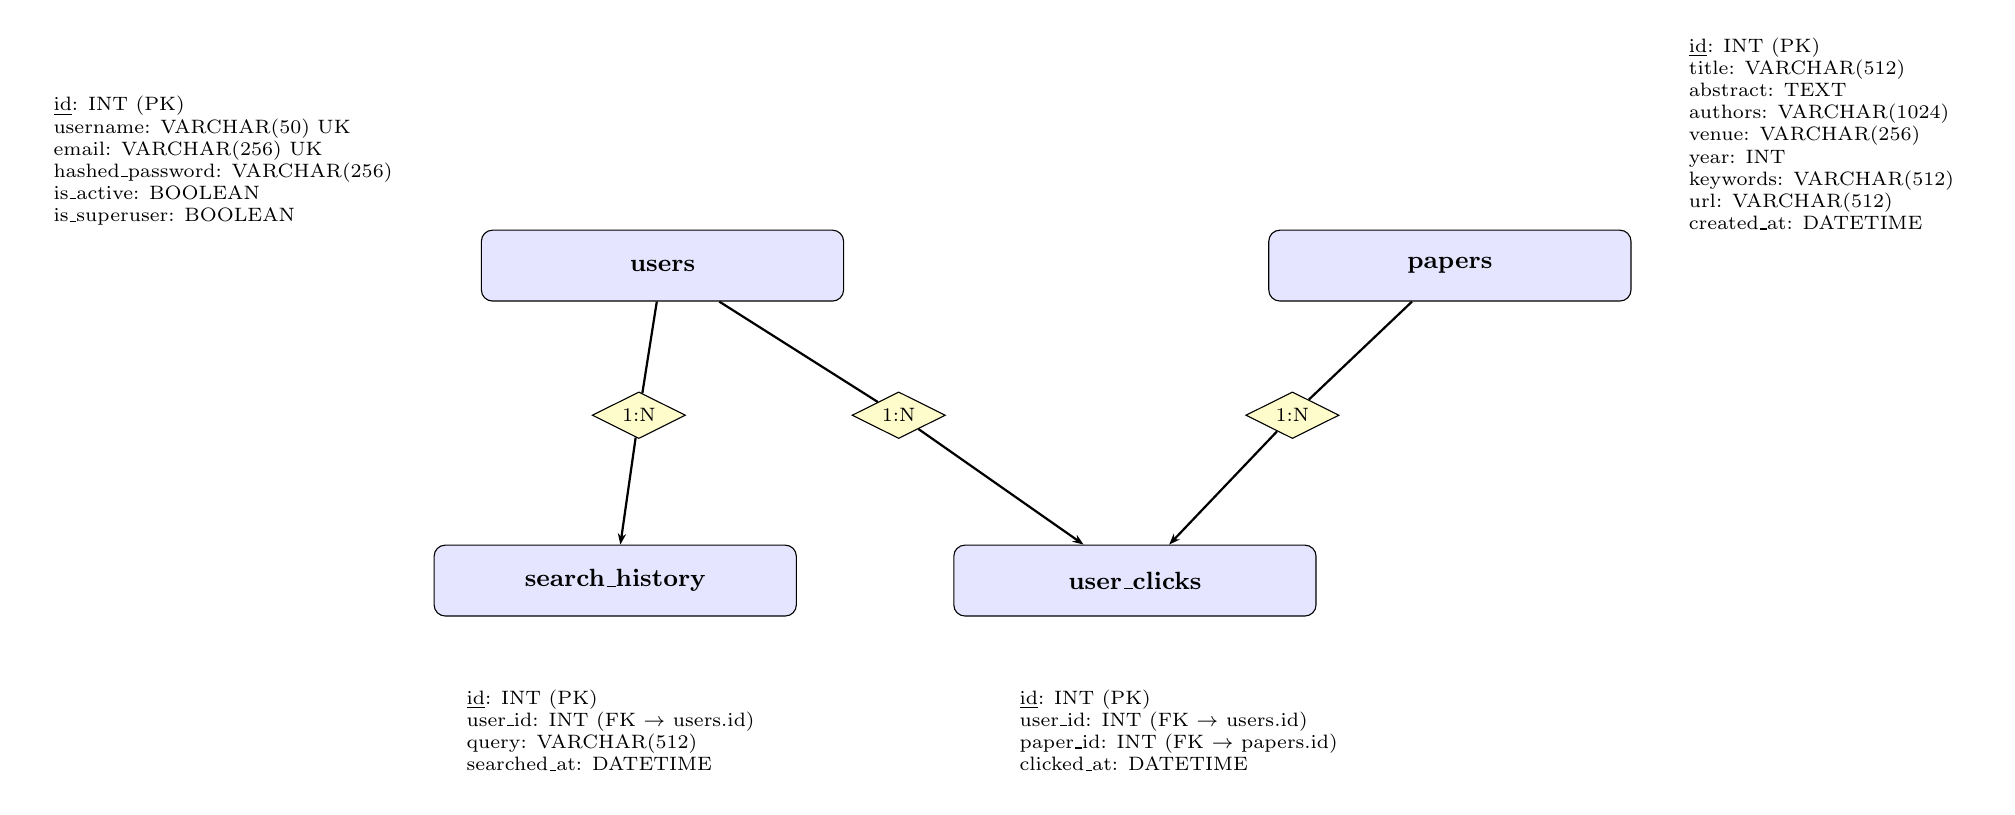
\begin{tikzpicture}[
    entity/.style={draw, rectangle, rounded corners=4pt, minimum width=4.6cm, minimum height=0.9cm, fill=blue!10, font=\small\bfseries},
    attr/.style={font=\scriptsize, align=left},
    rel/.style={draw, diamond, aspect=2, fill=yellow!20, font=\scriptsize, inner sep=2pt},
    arr/.style={-{Stealth[length=4pt]}, thick},
    line/.style={thick},
]

% Entities
\node[entity] (users) at (0, 0) {users};
\node[entity] (papers) at (10, 0) {papers};
\node[entity] (history) at (-0.6, -4) {search\_history};
\node[entity] (clicks) at (6.0, -4) {user\_clicks};

% Attributes - users
\node[attr, anchor=south east] at (-3.0, 0.35) {
  \begin{tabular}{l}
  \underline{id}: INT (PK) \\
  username: VARCHAR(50) UK \\
  email: VARCHAR(256) UK \\
  hashed\_password: VARCHAR(256) \\
  is\_active: BOOLEAN \\
  is\_superuser: BOOLEAN
  \end{tabular}
};

% Attributes - papers
\node[attr, anchor=south west] at (12.7, 0.25) {
  \begin{tabular}{l}
  \underline{id}: INT (PK) \\
  title: VARCHAR(512) \\
  abstract: TEXT \\
  authors: VARCHAR(1024) \\
  venue: VARCHAR(256) \\
  year: INT \\
  keywords: VARCHAR(512) \\
  url: VARCHAR(512) \\
  created\_at: DATETIME
  \end{tabular}
};

% Attributes - history
\node[attr, anchor=north east] at (1.6, -5.25) {
  \begin{tabular}{l}
  \underline{id}: INT (PK) \\
  user\_id: INT (FK $\to$ users.id) \\
  query: VARCHAR(512) \\
  searched\_at: DATETIME
  \end{tabular}
};

% Attributes - clicks
\node[attr, anchor=north west] at (4.2, -5.25) {
  \begin{tabular}{l}
  \underline{id}: INT (PK) \\
  user\_id: INT (FK $\to$ users.id) \\
  paper\_id: INT (FK $\to$ papers.id) \\
  clicked\_at: DATETIME
  \end{tabular}
};

% Relationships
\node[rel] (r1) at (3.0, -1.9) {1:N};
\node[rel] (r2) at (8.0, -1.9) {1:N};
\node[rel] (r3) at (-0.3, -1.9) {1:N};

\draw[line] (users) -- (r1);
\draw[arr] (r1) -- (clicks);
\draw[line] (papers) -- (r2);
\draw[arr] (r2) -- (clicks);
\draw[line] (users) -- (r3);
\draw[arr] (r3) -- (history);

\end{tikzpicture}
}
\caption{系统ER图}
\label{fig:er}
\end{figure}

\subsection{表结构详细设计}

\subsubsection{users — 用户表}

\begin{table}[H]
\centering
\caption{\code{users}表结构}
\begin{tabular}{lllp{5cm}}
\toprule
\textbf{字段} & \textbf{类型} & \textbf{约束} & \textbf{说明} \\
\midrule
\code{id}              & INT          & PK, AUTO\_INCREMENT & 主键 \\
\code{username}        & VARCHAR(50)  & UNIQUE, NOT NULL    & 登录用户名 \\
\code{email}           & VARCHAR(256) & UNIQUE, INDEX       & 邮箱地址 \\
\code{first\_name}     & VARCHAR(128) &                     & 名 \\
\code{last\_name}      & VARCHAR(128) &                     & 姓 \\
\code{hashed\_password}& VARCHAR(256) &                     & bcrypt加密密码 \\
\code{is\_active}      & BOOLEAN      & DEFAULT TRUE        & 账户激活状态 \\
\code{is\_superuser}   & BOOLEAN      & DEFAULT FALSE       & 管理员标志 \\
\bottomrule
\end{tabular}
\end{table}

\subsubsection{papers — 论文表}

\begin{table}[H]
\centering
\caption{\code{papers}表结构}
\begin{tabular}{lllp{5cm}}
\toprule
\textbf{字段} & \textbf{类型} & \textbf{约束} & \textbf{说明} \\
\midrule
\code{id}          & INT            & PK, AUTO\_INCREMENT & 主键 \\
\code{title}       & VARCHAR(512)   &                     & 论文标题 \\
\code{abstract}    & TEXT           &                     & 摘要 \\
\code{authors}     & VARCHAR(1024)  &                     & 作者（逗号分隔）\\
\code{venue}       & VARCHAR(256)   &                     & 发表会议/期刊 \\
\code{year}        & INT            &                     & 发表年份 \\
\code{keywords}    & VARCHAR(512)   &                     & 关键词（逗号分隔）\\
\code{url}         & VARCHAR(512)   &                     & 论文来源链接 \\
\code{created\_at} & DATETIME       & DEFAULT UTC\_NOW    & 入库时间 \\
\bottomrule
\end{tabular}
\end{table}

\subsubsection{user\_clicks — 点击记录表}

\begin{table}[H]
\centering
\caption{\code{user\_clicks}表结构}
\begin{tabular}{lllp{5cm}}
\toprule
\textbf{字段} & \textbf{类型} & \textbf{约束} & \textbf{说明} \\
\midrule
\code{id}          & INT      & PK, AUTO\_INCREMENT     & 主键 \\
\code{user\_id}    & INT      & FK $\to$ \code{users.id} & 点击用户 \\
\code{paper\_id}   & INT      & FK $\to$ \code{papers.id}& 被点击论文 \\
\code{clicked\_at} & DATETIME & DEFAULT UTC\_NOW         & 点击时间 \\
\bottomrule
\end{tabular}
\end{table}

\subsubsection{search\_history — 搜索历史表}

\begin{table}[H]
\centering
\caption{\code{search\_history}表结构}
\begin{tabular}{lllp{5cm}}
\toprule
\textbf{字段} & \textbf{类型} & \textbf{约束} & \textbf{说明} \\
\midrule
\code{id}           & INT          & PK, AUTO\_INCREMENT     & 主键 \\
\code{user\_id}     & INT          & FK $\to$ \code{users.id} & 搜索用户 \\
\code{query}        & VARCHAR(512) &                          & 查询文本 \\
\code{searched\_at} & DATETIME     & DEFAULT UTC\_NOW         & 搜索时间 \\
\bottomrule
\end{tabular}
\end{table}

\subsection{关系说明}

\begin{itemize}
\item \code{users} 1:N \code{user\_clicks}——一个用户可有多条点击记录。
\item \code{papers} 1:N \code{user\_clicks}——一篇论文可被多个用户点击。
\item \code{users} 1:N \code{search\_history}——一个用户可有多条搜索历史。
\item \code{user\_clicks}构成\code{users}与\code{papers}之间的\textbf{多对多关系}（附带时间戳的关联表）。
\end{itemize}


% ════════════════════════════════════════════════════
% 第四章：业务层实现
% ════════════════════════════════════════════════════
\section{业务层实现}

业务层基于FastAPI框架（端口8000），通过SQLAlchemy ORM操作MySQL，负责用户认证、论文CRUD、搜索/推荐代理以及LLM对话转发。

\subsection{用户认证}

系统采用\textbf{OAuth2 Bearer Token + JWT}方案：

\begin{enumerate}
\item 用户通过\api{POST /token}提交用户名和密码。
\item 后端使用\code{bcrypt}验证密码哈希，通过后生成JWT Token（HS256签名，有效期30分钟）。
\item 后续请求在\code{Authorization: Bearer <token>}头中携带Token。
\item 受保护接口通过\code{oauth2\_scheme}依赖注入自动解析并验证Token。
\end{enumerate}

\subsection{API接口设计}

\begin{table}[H]
\centering
\caption{业务层API接口}
\label{tab:api}
\small
\begin{tabular}{lllp{5.5cm}}
\toprule
\textbf{端点} & \textbf{方法} & \textbf{认证} & \textbf{说明} \\
\midrule
\multicolumn{4}{l}{\textit{认证与用户}} \\
\code{/token}                & POST & 否 & 登录，返回JWT \\
\code{/users/}               & POST & 否 & 注册 \\
\code{/users/me/}            & GET  & 是 & 当前用户信息 \\
\code{/users/}               & GET  & 是 & 用户列表（分页）\\
\code{/users/\{id\}}         & GET  & 是 & 按ID获取用户 \\
\code{/users/name/\{name\}}  & GET  & 是 & 按用户名获取 \\
\midrule
\multicolumn{4}{l}{\textit{论文管理}} \\
\code{/papers/}              & GET  & 是 & 论文列表（分页）\\
\code{/papers/\{id\}}        & GET  & 是 & 论文详情 \\
\code{/papers/bulk}          & POST & 是 & 批量导入 \\
\midrule
\multicolumn{4}{l}{\textit{搜索与推荐}} \\
\code{/search}               & POST & 是 & 语义搜索 + 降级SQL \\
\code{/click}                & POST & 是 & 记录论文点击 \\
\code{/recommend}            & GET  & 是 & 个性化推荐 \\
\code{/search/history}       & GET  & 是 & 搜索历史 \\
\midrule
\multicolumn{4}{l}{\textit{AI对话}} \\
\code{/chat}                 & POST & 是 & 非流式LLM对话 \\
\code{/chat/stream}          & POST & 是 & 流式SSE对话（论文问答/RAG/纯对话）\\
\midrule
\multicolumn{4}{l}{\textit{PDF管理}} \\
\code{/papers/\{id\}/pdf}       & GET  & 是 & 下载论文PDF \\
\code{/papers/\{id\}/upload-pdf}& POST & 是 & 上传PDF（管理员）\\
\bottomrule
\end{tabular}
\end{table}

\subsection{核心业务逻辑}

\subsubsection{搜索代理与降级}

\api{POST /search}接口接收用户查询后：
\begin{enumerate}
\item 将查询记录写入\code{search\_history}表。
\item 将请求转发至算法层\api{/search}端点，附带\code{query}、\code{use\_rerank}、\code{rerank\_provider}、\code{recall\_k}等参数。
\item 算法层返回\code{paper\_id + score}列表后，业务层从MySQL批量查询论文元数据并拼接。
\item 若算法层不可用，则降级为SQL \code{LIKE}搜索（匹配\code{title}、\code{abstract}、\code{keywords}、\code{authors}字段）。
\end{enumerate}

\subsubsection{推荐代理}

\api{GET /recommend}接口：
\begin{enumerate}
\item 从\code{user\_clicks}表查询当前用户最近50条点击记录。
\item 将已点击论文ID列表发送至算法层\api{/recommend}端点。
\item 算法层返回推荐结果后，业务层从MySQL补全元数据返回前端。
\end{enumerate}

\subsubsection{对话上下文注入与RAG}

\api{POST /chat/stream}接口支持三种模式，由请求参数\code{paper\_id}和\code{use\_rag}控制：

\begin{enumerate}
\item \textbf{论文问答模式}（\code{paper\_id}有值）：调用算法层\api{/search-chunks}检索该论文全文分块（Top-5），将论文元信息与全文片段注入系统提示词，LLM基于论文实际内容回答。
\item \textbf{RAG全库模式}（\code{use\_rag=true}，默认）：以用户最后一条消息为查询，调用\api{/search-chunks}检索全库最相关的8个分块，按\code{paper\_id}聚合后注入上下文，同时构建引用列表。SSE流结束后发送\code{references}事件，前端显示可点击的参考论文标签。
\item \textbf{纯对话模式}（\code{use\_rag=false}）：保留原有逻辑，仅注入用户最近5篇已读论文摘要。
\end{enumerate}


% ════════════════════════════════════════════════════
% 第五章：算法层实现
% ════════════════════════════════════════════════════
\section{算法层实现}

算法层作为独立的FastAPI微服务（端口8003），封装了向量检索、推荐和对话三大核心算法。

\subsection{向量语义检索}

\subsubsection{索引构建}

对每篇论文 $p_i$，拼接其标题、摘要和关键词构成文档文本，通过\code{text-embedding-v4}模型生成1024维向量，存入ChromaDB：

\begin{equation}
\text{doc}_i = \text{concat}(p_i.\text{title},\ ".\ ",\ p_i.\text{abstract},\ ".\ ",\ p_i.\text{keywords})
\end{equation}
\begin{equation}
\mathbf{e}_i = \text{text-embedding-v4}(\text{doc}_i) \in \mathbb{R}^{1024}
\end{equation}

Embedding采用批量请求（每批最多10条），通过DashScope OpenAI兼容接口调用。

\subsubsection{检索流程}

给定查询文本$q$和返回数量$k$：
\begin{enumerate}
\item 将查询向量化：$\mathbf{q} = \text{text-embedding-v4}(q)$
\item ChromaDB ANN近邻搜索，返回Top-$k$结果及距离 $d_i$
\item 将距离转换为相关性分数：$\text{score}_i = \frac{1}{1 + d_i}$
\item 按分数降序返回
\end{enumerate}

\subsection{基于Embedding质心的推荐算法}

给定用户$u$的点击历史 $C = \{c_1, c_2, \dots, c_m\}$（最近50篇）和推荐数量$k$：

\begin{enumerate}
\item 从ChromaDB获取已点击论文的Embedding：$E = \{\mathbf{e}(c_1), \dots, \mathbf{e}(c_m)\}$
\item 计算兴趣质心：
\begin{equation}
\mathbf{centroid} = \frac{1}{m} \sum_{i=1}^{m} \mathbf{e}(c_i)
\end{equation}
\item 以质心向量查询ChromaDB，获取$k + |C|$个候选
\item 过滤已读论文，返回前$k$个
\end{enumerate}

该方法本质上是\textbf{基于内容的协同过滤}——质心方向代表用户的综合兴趣方向，实时计算，无需离线训练。

\subsection{Reranker精排}

系统支持三种精排策略：

\begin{enumerate}
\item \textbf{无精排}（\code{none}）：直接返回ChromaDB的距离排序结果。
\item \textbf{余弦相似度重排}（\code{cosine}）：对查询和候选文档统一进行Embedding，L2归一化后计算余弦相似度：
\begin{equation}
\text{score}_i = \frac{\mathbf{q} \cdot \mathbf{d}_i}{\|\mathbf{q}\| \cdot \|\mathbf{d}_i\|}
\end{equation}
\item \textbf{Qwen3-Rerank}（\code{qwen}）：调用DashScope的\code{qwen3-rerank}模型，对查询和候选文档进行交叉编码精排，效果最优但延迟较高。
\end{enumerate}

\subsection{PDF全文提取与分块Embedding}

为使LLM能够基于论文全文内容回答问题，系统实现了PDF全文提取与分块Embedding管道：

\subsubsection{全文提取}

使用PyMuPDF（\code{fitz}）逐页提取PDF文本。对120篇论文PDF进行处理，共提取约2080个文本分块。

\subsubsection{分块策略}

采用滑动窗口分块：每块约800词，相邻块重叠100词，确保上下文连续性：

\begin{equation}
\text{chunks} = \{\text{words}[i:i+800] \mid i = 0, 700, 1400, \dots\}
\end{equation}

对超长文本（如含编码数据的PDF），在Embedding前截断至8000字符以满足API输入限制。

\subsubsection{向量索引}

分块文本通过\code{text-embedding-v4}生成1024维向量，存入ChromaDB的\code{paper\_chunks} collection，每个分块附带\code{paper\_id}和\code{chunk\_index}元数据，支持按论文ID过滤检索：

\begin{lstlisting}[language=Python, caption=分块索引数据结构]
collection.upsert(
    ids=["paper_42_chunk_3"],
    documents=["chunk text..."],
    embeddings=[...],        # 1024-dim vector
    metadatas=[{"paper_id": 42, "chunk_index": 3}],
)
\end{lstlisting}

算法层提供两个新端点：
\begin{itemize}
\item \api{POST /index-chunks}：批量索引分块（提取脚本调用）
\item \api{POST /search-chunks}：检索分块，支持\code{paper\_id}过滤（全库或单篇论文检索）
\end{itemize}

\subsection{LLM学术问答与RAG}

通过DashScope OpenAI兼容接口调用\code{qwen-flash}模型，支持流式和非流式两种模式。

\subsubsection{论文问答}

在论文详情页，用户可直接提问。系统从该论文的全文分块中检索最相关的5个片段注入系统提示词，使LLM能基于论文实际全文内容（而非仅摘要）回答问题。

\subsubsection{RAG全库检索增强生成}

在AI对话页面，系统以用户问题为查询从全库2080个分块中检索Top-8最相关片段，按论文ID聚合后注入系统提示词，并生成引用列表。LLM回答后，前端显示参考论文标签，用户可点击跳转至对应论文详情页。

流式响应通过FastAPI \code{StreamingResponse}实现SSE推送。


% ════════════════════════════════════════════════════
% 第六章：前端界面实现
% ════════════════════════════════════════════════════
\section{前端界面实现}

前端基于Vue~3 Composition API + Element Plus构建，通过Vite开发服务器代理\code{/api/*}请求至业务后端。

\subsection{页面组成}

\begin{table}[H]
\centering
\caption{前端页面与功能}
\begin{tabular}{llp{7cm}}
\toprule
\textbf{页面} & \textbf{组件} & \textbf{功能说明} \\
\midrule
登录      & \code{LoginForm.vue}     & 用户名密码登录，JWT持久化到localStorage \\
注册      & \code{RegisterForm.vue}  & 新用户注册（用户名、邮箱、姓名）\\
论文搜索  & \code{PaperSearch.vue}   & 语义搜索 + 搜索历史标签 + Rerank开关 + 分页 \\
论文详情  & \code{PaperDetail.vue}   & 标题、摘要、PDF阅读器、\textbf{AI论文问答} \\
论文推荐  & \code{PaperRecommend.vue}& 基于浏览历史的个性化推荐列表 \\
AI对话    & \code{Chat.vue}          & SSE流式渲染 + \textbf{RAG检索增强} + 参考论文 \\
用户管理  & \code{Profile.vue}等     & 个人信息、用户列表、添加用户 \\
\bottomrule
\end{tabular}
\end{table}

\subsection{关键前端特性}

\begin{itemize}
\item \textbf{路由守卫}：通过\code{vue-router}的\code{beforeEach}钩子，未登录用户自动重定向至登录页。
\item \textbf{Token持久化}：JWT存储在\code{localStorage}，Axios拦截器自动注入\code{Authorization}头。
\item \textbf{流式渲染}：AI对话使用\code{fetch} + \code{ReadableStream}接收SSE，通过\code{marked}库实时渲染Markdown。
\item \textbf{论文问答}：论文详情页内嵌AI问答框，提供快捷提问（"核心方法"、"主要贡献"等），基于论文全文分块回答。
\item \textbf{RAG参考引用}：AI对话页自动检索全库论文分块，回答后显示参考论文标签，点击可跳转至对应详情页。
\item \textbf{搜索历史}：去重后以Element Plus Tag组件展示，点击标签可快速复搜。
\item \textbf{Rerank开关}：搜索页面提供精排开关，设置持久化到\code{localStorage}。
\item \textbf{状态管理}：使用Pinia管理用户状态，支持Token自动恢复。
\end{itemize}

\subsection{路由设计}

\begin{table}[H]
\centering
\caption{前端路由表}
\begin{tabular}{lll}
\toprule
\textbf{路径} & \textbf{组件} & \textbf{说明} \\
\midrule
\code{/}                       & Login.vue           & 登录页 \\
\code{/register}               & Register.vue        & 注册页 \\
\code{/index}                  & Index.vue           & 主布局（Header + 侧边栏）\\
\code{/index/paperSearch}      & PaperSearch.vue     & 论文搜索 \\
\code{/index/paperDetail/:id}  & PaperDetail.vue     & 论文详情 \\
\code{/index/paperRecommend}   & PaperRecommend.vue  & 论文推荐 \\
\code{/index/chat}             & Chat.vue            & AI对话 \\
\code{/index/checkUserInfo}    & CheckUserInfo.vue   & 用户管理 \\
\bottomrule
\end{tabular}
\end{table}


% ════════════════════════════════════════════════════
% 第七章：算法分析与实验
% ════════════════════════════════════════════════════
\section{算法分析与实验}

\subsection{实验环境}

\begin{itemize}
\item \textbf{数据集}：120篇来自OpenAlex的真实数据库/数据管理领域论文（含标题、摘要、关键词）
\item \textbf{Embedding模型}：\code{text-embedding-v4}（1024维），DashScope API
\item \textbf{向量数据库}：ChromaDB（persistent模式）
\item \textbf{Ground Truth}：基于8个主题类别构建20条搜索查询及对应相关论文标注
\item \textbf{重复次数}：每组实验重复3次取均值
\end{itemize}

\subsection{评估指标}

\begin{table}[H]
\centering
\caption{评估指标定义}
\begin{tabular}{lp{10cm}}
\toprule
\textbf{指标} & \textbf{定义} \\
\midrule
P@K      & 前$K$个结果中相关文档的比例 \\
R@K      & 前$K$个结果覆盖的召回率 \\
MRR      & 第一个相关结果的排名倒数的均值 \\
NDCG@K   & 归一化折损累积增益，考虑排序位置的加权指标 \\
MAP      & 各查询Average Precision的均值 \\
Hit Rate@K & 推荐的$K$篇中是否包含目标论文 \\
Coverage & 推荐结果覆盖的论文比例 \\
Diversity & 推荐列表内部两两余弦距离的均值 \\
Novelty  & 推荐物品的平均自信息量 \\
\bottomrule
\end{tabular}
\end{table}

\subsection{实验一：搜索系统消融实验}

逐一替换或移除系统组件，评估各组件对搜索效果的贡献。

\begin{table}[H]
\centering
\caption{搜索系统消融实验结果}
\label{tab:search_ablation}
\small
\begin{tabular}{clcccccc}
\toprule
\textbf{编号} & \textbf{配置} & \textbf{P@5} & \textbf{P@10} & \textbf{P@20} & \textbf{NDCG@5} & \textbf{MRR} & \textbf{延迟(ms)} \\
\midrule
A1 & 完整系统（向量+Rerank）& 0.825 & 0.713 & 0.513 & 0.847 & 0.958 & 467.7 \\
A2 & SQL LIKE关键词搜索     & 0.542 & 0.508 & 0.396 & 0.546 & 0.690 & 7.3 \\
A3 & TF-IDF余弦相似度       & 0.725 & 0.646 & 0.513 & 0.753 & 0.872 & 0.5 \\
A4 & 向量检索（无Rerank）    & 0.825 & 0.713 & 0.513 & 0.847 & 0.958 & 186.1 \\
A5 & 向量检索（余弦距离）    & 0.825 & 0.713 & 0.513 & 0.847 & 0.958 & 250.1 \\
\bottomrule
\end{tabular}
\end{table}

\textbf{分析}：向量语义检索（A1/A4/A5）在P@K和NDCG@K上显著优于SQL LIKE（A2），P@5提升52.2\%（0.542$\to$0.825）。TF-IDF（A3）效果居中但在P@10上弱于向量检索（0.646 vs 0.713），说明预训练Embedding在语义理解上有明显优势。Rerank对Top-K指标无额外贡献（A1与A4一致），但引入约280ms额外延迟。

\begin{figure}[H]
\centering
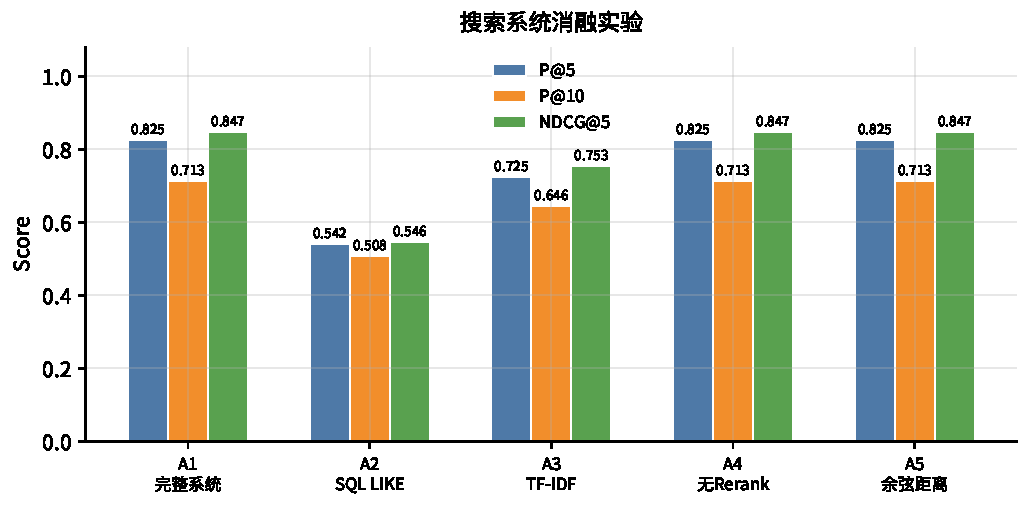
\includegraphics[width=0.85\textwidth]{search_ablation.pdf}
\caption{搜索系统消融实验：各配置在P@5、P@10、NDCG@5上的对比}
\label{fig:search_ablation}
\end{figure}

\subsection{实验二：推荐系统消融实验}

\begin{table}[H]
\centering
\caption{推荐系统消融实验结果}
\label{tab:rec_ablation}
\begin{tabular}{clcccc}
\toprule
\textbf{编号} & \textbf{配置} & \textbf{Hit Rate@10} & \textbf{Coverage} & \textbf{Diversity} & \textbf{延迟(ms)} \\
\midrule
B1 & 完整质心推荐       & 0.727 & 0.542 & 0.494 & 4.9 \\
B2 & 仅最后一次点击推荐 & 0.682 & 0.658 & 0.508 & 4.8 \\
B3 & 缩短窗口（5篇）    & 0.727 & 0.542 & 0.494 & 4.8 \\
B4 & 不过滤已读         & 0.682 & 0.625 & 0.490 & 4.8 \\
B5 & 质心加随机扰动     & 0.591 & 0.742 & 0.533 & 4.9 \\
\bottomrule
\end{tabular}
\end{table}

\textbf{分析}：多篇点击的质心推荐（B1）优于仅用最后一篇（B2），Hit Rate提升6.6\%（0.682$\to$0.727）。随机扰动（B5）牺牲了命中率但显著提高了Coverage和Diversity，体现了精准与探索的经典权衡。

\begin{figure}[H]
\centering
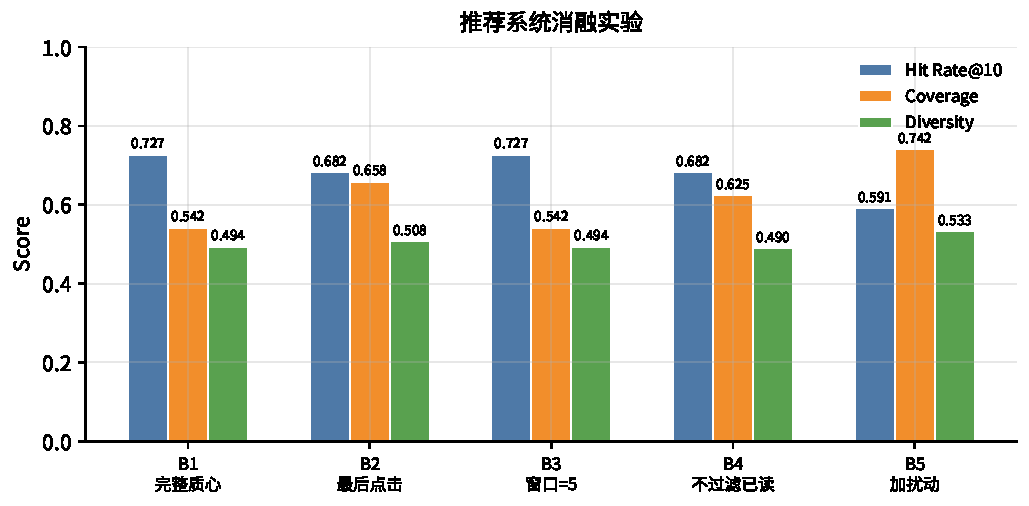
\includegraphics[width=0.85\textwidth]{recommend_ablation.pdf}
\caption{推荐系统消融实验：各配置在Hit Rate@10、Coverage、Diversity上的对比}
\label{fig:recommend_ablation}
\end{figure}

\subsection{实验三：搜索系统性能评估}

\begin{table}[H]
\centering
\caption{搜索系统完整性能评估（3次重复）}
\begin{tabular}{lccccc}
\toprule
\textbf{指标} & \textbf{P@5} & \textbf{P@10} & \textbf{P@20} & \textbf{MRR} & \textbf{MAP} \\
\midrule
均值 & 0.825 & 0.713 & 0.513 & 0.958 & 0.447 \\
\bottomrule
\end{tabular}

\vspace{0.5em}

\caption{搜索延迟分解（ms）}
\begin{tabular}{lcc}
\toprule
\textbf{阶段} & \textbf{均值} & \textbf{标准差} \\
\midrule
Embedding编码     & 202.2 & 19.5 \\
ChromaDB检索      & 6.1   & 0.6 \\
Reranker精排      & 8.6   & 0.6 \\
\textbf{端到端总计} & \textbf{217.0} & \textbf{19.0} \\
\bottomrule
\end{tabular}
\end{table}

\textbf{分析}：延迟瓶颈主要在Embedding编码（占93.2\%），ChromaDB向量检索本身仅需约6ms。标准差较小（19.0ms），说明系统延迟稳定。

\begin{figure}[H]
\centering
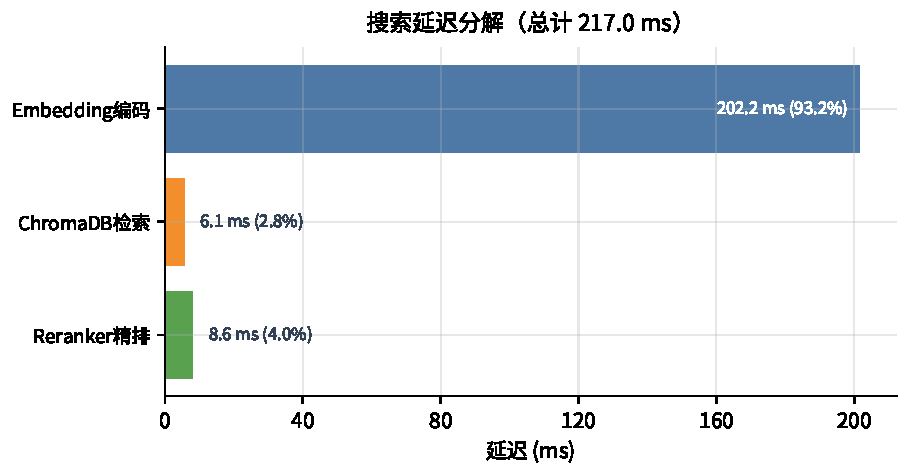
\includegraphics[width=0.55\textwidth]{latency_breakdown.pdf}
\caption{搜索延迟分解：Embedding编码占端到端延迟的93.2\%}
\label{fig:latency_breakdown}
\end{figure}

\subsection{实验四：推荐系统性能评估}

\begin{table}[H]
\centering
\caption{推荐系统性能评估}
\begin{tabular}{lccccc}
\toprule
\textbf{指标} & \textbf{Hit Rate@10} & \textbf{Coverage} & \textbf{Diversity} & \textbf{Novelty} & \textbf{延迟(ms)} \\
\midrule
均值 & 0.591 & 0.542 & 0.494 & 6.644 & 4.9 \\
\bottomrule
\end{tabular}
\end{table}

\subsection{实验五：距离度量对比}

\begin{table}[H]
\centering
\caption{不同距离度量的检索效果}
\begin{tabular}{lcccccc}
\toprule
\textbf{距离度量} & \textbf{P@5} & \textbf{P@10} & \textbf{NDCG@5} & \textbf{NDCG@10} & \textbf{MRR} & \textbf{延迟(ms)} \\
\midrule
L2 欧氏距离    & 0.825 & 0.713 & 0.847 & 0.760 & 0.958 & 3.64 \\
Cosine 余弦    & 0.825 & 0.713 & 0.847 & 0.760 & 0.958 & 3.75 \\
Inner Product  & 0.825 & 0.713 & 0.847 & 0.760 & 0.958 & 4.89 \\
\bottomrule
\end{tabular}
\end{table}

\textbf{分析}：在\code{text-embedding-v4}生成的归一化向量上，三种度量效果完全一致——对归一化向量，L2距离、余弦相似度和内积在排序上数学等价。

\subsection{实验六：文档表示对比}

\begin{table}[H]
\centering
\caption{不同文档表示方式的检索效果}
\label{tab:doc_repr}
\begin{tabular}{clccccc}
\toprule
\textbf{编号} & \textbf{文档表示} & \textbf{P@5} & \textbf{P@10} & \textbf{NDCG@5} & \textbf{MRR} & \textbf{MAP} \\
\midrule
C1 & 仅Title                    & 0.692 & 0.600 & 0.732 & 0.931 & 0.371 \\
C2 & 仅Abstract                 & \textbf{0.850} & 0.683 & \textbf{0.863} & 0.938 & 0.420 \\
C3 & 仅Keywords                 & 0.767 & 0.629 & 0.807 & 0.958 & 0.381 \\
C4 & Title + Abstract           & 0.833 & 0.696 & 0.854 & 0.958 & 0.432 \\
C5 & Title + Abstract + Keywords& 0.825 & \textbf{0.713} & 0.847 & \textbf{0.958} & \textbf{0.447} \\
\bottomrule
\end{tabular}
\end{table}

\textbf{分析}：仅Abstract（C2）在P@5和NDCG@5上最高（0.850、0.863），但完整拼接（C5）在P@10和MAP上最优（0.713、0.447），综合表现最均衡，故作为系统默认配置。仅Title（C1）效果最差，说明标题信息量有限。

\begin{figure}[H]
\centering
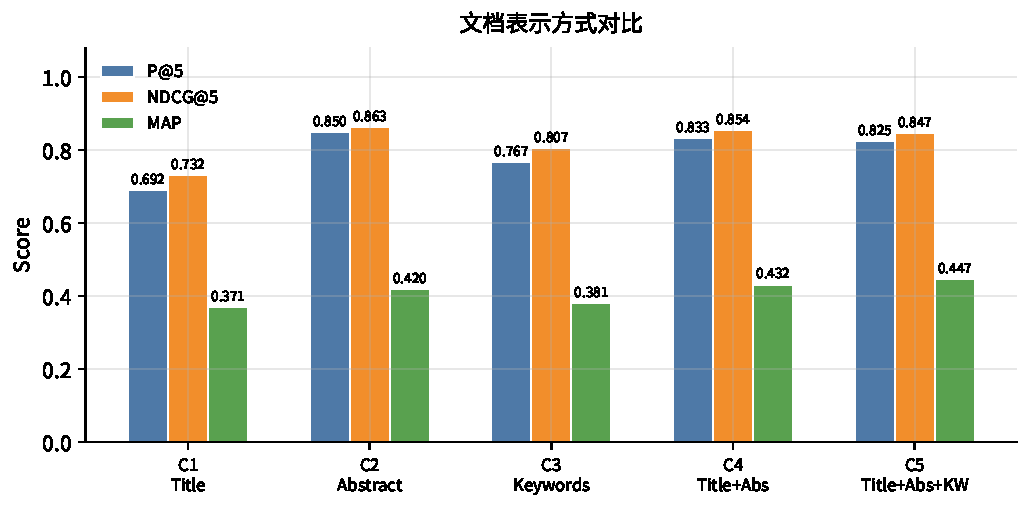
\includegraphics[width=0.85\textwidth]{doc_representation.pdf}
\caption{文档表示方式对比：不同字段组合在P@5、NDCG@5、MAP上的表现}
\label{fig:doc_repr}
\end{figure}

\subsection{实验七：Reranker对比}

\begin{table}[H]
\centering
\caption{不同Reranker策略的效果}
\begin{tabular}{clcccccc}
\toprule
\textbf{编号} & \textbf{Pipeline} & \textbf{P@5} & \textbf{P@10} & \textbf{NDCG@5} & \textbf{MAP} & \textbf{延迟(ms)} \\
\midrule
R1 & Base Vector（无精排）      & 0.825 & \textbf{0.713} & 0.847 & 0.447 & 259.7 \\
R2 & Qwen3-Rerank（召回60）     & \textbf{0.833} & 0.663 & 0.846 & 0.447 & 602.7 \\
R3 & Qwen3-Rerank（召回100）    & 0.825 & 0.679 & 0.841 & \textbf{0.451} & 678.5 \\
\bottomrule
\end{tabular}
\end{table}

\textbf{分析}：Qwen3-Rerank在P@5上微幅提升（R2=0.833 vs R1=0.825），但P@10反而下降（0.663 vs 0.713），且延迟翻倍（\textasciitilde 603ms vs 260ms）。扩大召回窗口（R3 vs R2）效果无明显差异，说明60的召回量已足够。在当前数据集上，Rerank的精度增益有限，但延迟代价显著。

\begin{figure}[H]
\centering
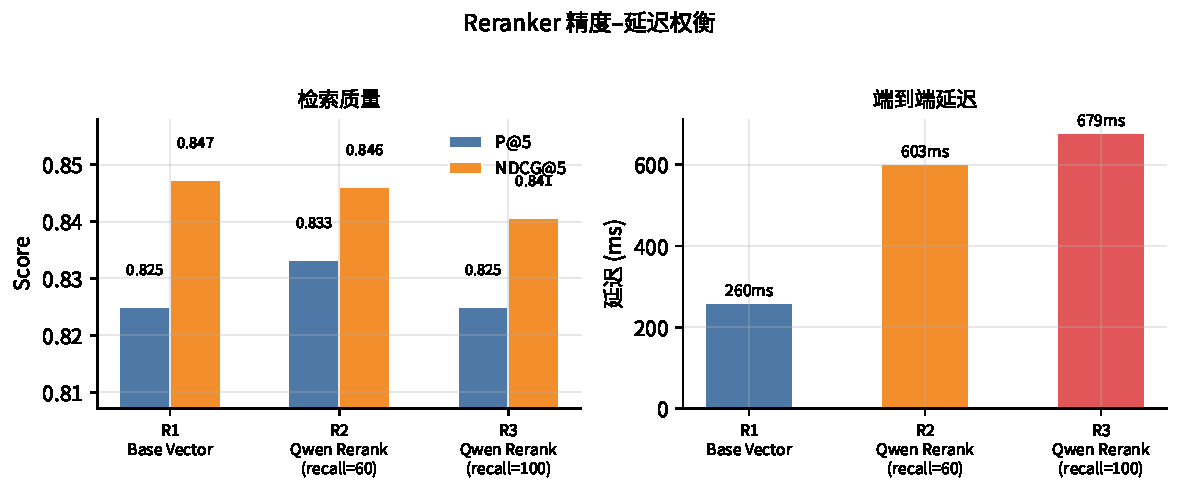
\includegraphics[width=0.9\textwidth]{reranker_tradeoff.pdf}
\caption{Reranker精度–延迟权衡：精排提升P@5约2.5\%，但延迟增加约一倍}
\label{fig:reranker_tradeoff}
\end{figure}

\subsection{实验八：数据规模扩展测试}

\begin{table}[H]
\centering
\caption{不同数据规模下的性能}
\begin{tabular}{rrrrrr}
\toprule
\textbf{论文数} & \textbf{索引构建(ms)} & \textbf{Embedding(ms)} & \textbf{平均查询(ms)} & \textbf{P95(ms)} & \textbf{Max(ms)} \\
\midrule
20  & 1,287  & 1,176  & 2.60 & 3.56 & 4.42 \\
40  & 2,818  & 2,682  & 2.76 & 4.03 & 5.24 \\
60  & 4,037  & 3,876  & 3.66 & 8.62 & 11.41 \\
80  & 5,212  & 4,960  & 2.80 & 4.18 & 5.48 \\
100 & 6,376  & 6,179  & 2.89 & 4.44 & 5.89 \\
120 & 8,228  & 7,994  & 2.84 & 4.58 & 6.27 \\
\bottomrule
\end{tabular}
\end{table}

\textbf{分析}：索引构建时间与论文数量呈线性关系，瓶颈在Embedding编码（API调用），ChromaDB upsert仅占约3\%。查询延迟在120篇规模下稳定在2.6--3.7ms（均值），表明系统具有良好的可扩展性。

\begin{figure}[H]
\centering
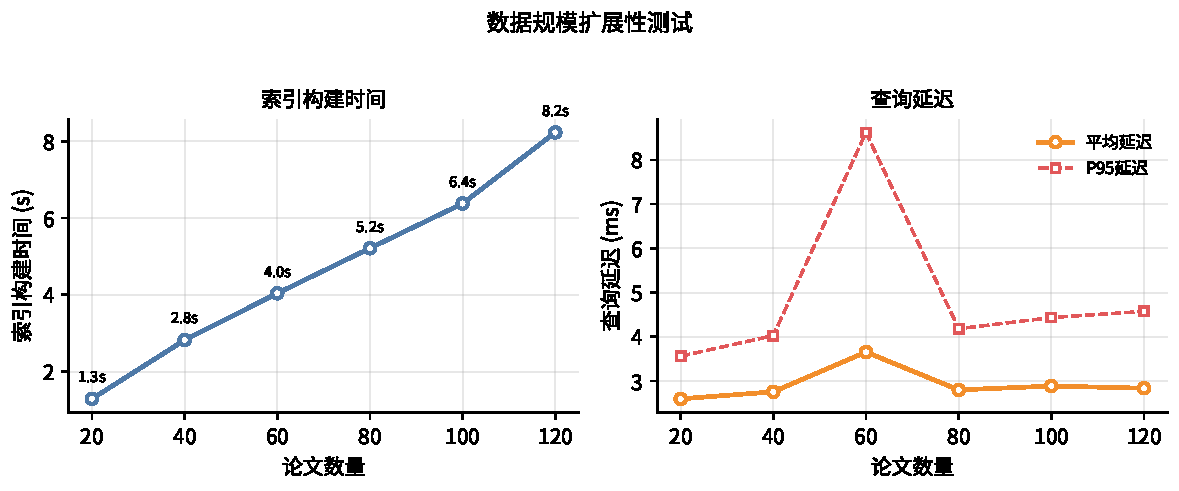
\includegraphics[width=0.9\textwidth]{scalability.pdf}
\caption{数据规模扩展性测试：索引构建时间线性增长，查询延迟稳定在2.6--3.7ms}
\label{fig:scalability}
\end{figure}

\subsection{实验小结}

\begin{enumerate}
\item 向量语义检索相比SQL LIKE，P@5提升52.2\%（0.542 $\to$ 0.825），语义理解能力显著。
\item 质心推荐比仅用最后一篇点击Hit Rate提升6.6\%（0.682$\to$0.727），多篇历史有助于捕捉综合兴趣。
\item 系统端到端搜索延迟约217ms，瓶颈在Embedding编码（93.2\%），ChromaDB检索本身仅约6ms。
\item Qwen3-Rerank在当前数据集上精度增益有限（P@5+0.8\%），但延迟增加约一倍，适合对精度要求极高的场景。
\item 归一化向量下L2/Cosine/IP三种度量效果完全等价。
\item 完整的Title+Abstract+Keywords拼接在P@10和MAP上最优，是最均衡的文档表示方式。
\end{enumerate}


% ════════════════════════════════════════════════════
% 第八章：测试数据
% ════════════════════════════════════════════════════
\section{测试数据}

\subsection{论文数据集}

系统使用120篇来自OpenAlex的真实学术论文作为种子数据，涵盖数据库与数据管理领域的多个方向：

\begin{itemize}
\item 查询优化（Query Optimization）
\item SQL索引（SQL Indexing）
\item 分布式数据库（Distributed Database）
\item 事务处理（Transaction Processing）
\item 图数据库（Graph Database）
\item 云数据库（Cloud Database）
\item 安全与隐私（Security \& Privacy）
\item 信息检索与索引（Retrieval \& Indexing）
\end{itemize}

每篇论文包含标题、完整摘要、作者列表、发表会议/期刊、年份、关键词和来源链接，数据来源为OpenAlex学术API。此外，系统本地存储了120篇论文的PDF全文（约187MB），通过PyMuPDF提取文本后分块Embedding，共生成约2080个全文分块向量，用于论文问答和RAG检索增强。

\subsection{Ground Truth构建}

搜索实验的Ground Truth基于主题规则自动生成：

\begin{enumerate}
\item 定义8个主题类别，每个类别包含若干关键词规则。
\item 设计20条接近真实用户意图的搜索查询（非简单论文标题复制）。
\item 论文按摘要和关键词与主题规则的匹配度标注为相关/不相关。
\item 每条查询标注关联的\code{focus}关键词，用于生成分级相关度。
\end{enumerate}

\subsection{推荐评估数据}

推荐实验的评估数据基于模拟用户行为构建：
\begin{enumerate}
\item 按主题类别将论文分组，为每个主题模拟2--3个用户Session。
\item 每个Session包含5--10次点击历史（同主题论文）。
\item 使用Leave-One-Out方法：保留最后一篇作为目标，用前$n-1$篇生成推荐。
\end{enumerate}


% ════════════════════════════════════════════════════
% 第九章：用户手册
% ════════════════════════════════════════════════════
\section{用户手册}

\subsection{环境要求}

\begin{itemize}
\item Python 3.10+
\item Node.js 18+
\item MySQL 8.0+
\item DashScope API Key（用于Embedding和LLM）
\end{itemize}

\subsection{安装与配置}

\begin{lstlisting}[language=bash, caption=安装依赖]
# 克隆仓库
git clone git@github.com:JunjieNian/paper-search-database.git
cd paper-search-database

# Python 环境
python3 -m venv .venv
source .venv/bin/activate
pip install -r backend/requirements.txt
pip install -r backend_algo/requirements.txt

# 前端依赖
cd frontend && npm install && cd ..
\end{lstlisting}

\begin{lstlisting}[language=bash, caption=配置环境变量]
cp backend/.env.example backend/.env
cp backend_algo/.env.example backend_algo/.env
cp frontend/.env.development.example frontend/.env.development.local

# 编辑 backend/.env: 填写 MYSQL_USER, MYSQL_PASSWORD
# 编辑 backend_algo/.env: 填写 DASHSCOPE_API_KEY
\end{lstlisting}

\begin{lstlisting}[language=sql, caption=创建数据库]
CREATE DATABASE paper_search CHARACTER SET utf8mb4;
\end{lstlisting}

\subsection{启动服务}

\textbf{方式一：一键启动（推荐）}
\begin{lstlisting}[language=bash]
bash start_all.sh     # 启动全部服务
bash stop_all.sh      # 停止全部服务
\end{lstlisting}

\textbf{方式二：手动启动}
\begin{lstlisting}[language=bash]
# 终端1: 算法层
cd backend_algo && python -m uvicorn main:app --host 0.0.0.0 --port 8003

# 终端2: 业务后端
cd backend && python -m uvicorn main:app --host 0.0.0.0 --port 8000

# 终端3: 前端
cd frontend && npm run dev -- --host 0.0.0.0
\end{lstlisting}

\subsection{导入种子数据}

\begin{lstlisting}[language=bash]
cd backend && python seed_papers.py       # 导入论文元数据+摘要索引
cd backend && python extract_chunks.py    # PDF全文提取+分块索引
\end{lstlisting}

\code{seed\_papers.py}将120篇论文写入MySQL并在ChromaDB中建立摘要级向量索引。\code{extract\_chunks.py}使用PyMuPDF提取PDF全文，按800词/块分块后通过算法层\api{/index-chunks}建立全文分块索引（约2080个chunks），支持后续的论文问答和RAG检索。

\subsection{功能使用}

\begin{enumerate}
\item \textbf{注册与登录}：打开\code{http://localhost:5173}，点击注册创建账户，然后登录。
\item \textbf{论文搜索}：在侧边栏点击"论文搜索"，输入自然语言查询（如"query optimization in distributed databases"），点击搜索。支持切换是否启用Rerank精排。
\item \textbf{查看论文}：点击搜索结果中的论文标题，查看论文详情（标题、作者、摘要、PDF全文）。
\item \textbf{论文问答}：在论文详情页底部的"AI论文问答"区域，可以直接就该论文提问（如"核心方法"、"主要贡献"），AI基于论文全文分块回答。
\item \textbf{论文推荐}：浏览若干论文后，点击侧边栏"论文推荐"，系统将根据浏览历史推荐相关论文。
\item \textbf{AI对话}：点击侧边栏"AI对话"，与LLM进行多轮学术问答。系统自动检索全库论文全文分块（RAG），回答后显示参考论文标签，点击标签可跳转至对应论文详情。
\item \textbf{搜索历史}：搜索页面上方显示去重后的搜索历史标签，点击可快速复搜。
\end{enumerate}

\subsection{访问地址}

\begin{table}[H]
\centering
\begin{tabular}{ll}
\toprule
\textbf{服务} & \textbf{地址} \\
\midrule
前端界面        & \code{http://localhost:5173} \\
业务层API文档   & \code{http://localhost:8000/docs} \\
算法层API文档   & \code{http://localhost:8003/docs} \\
\bottomrule
\end{tabular}
\end{table}

\subsection{运行实验}

\begin{lstlisting}[language=bash]
cd experiments
pip install -r requirements.txt
python run_all.py                    # 运行实验 1-8
RUN_CONCURRENT=1 python run_all.py   # 包含并发压测
\end{lstlisting}

实验结果以JSON格式保存在\code{experiments/results/}目录。


% ════════════════════════════════════════════════════
% 第十章：项目结构
% ════════════════════════════════════════════════════
\section{项目结构}

\begin{lstlisting}[basicstyle=\small\ttfamily, frame=none, numbers=none, xleftmargin=0em]
mysql_fastapi_vue_project/
|-- frontend/                     # 前端 (Vue 3 + Element Plus)
|   |-- src/
|   |   |-- router/index.ts       # 路由 + 登录守卫
|   |   |-- store/user.ts         # Pinia 状态管理
|   |   |-- request/api.ts        # API 接口封装
|   |   |-- components/           # 业务组件
|   |   `-- pages/                # 页面组件
|   `-- vite.config.ts            # 构建配置 + 代理
|
|-- backend/                      # 业务层 (FastAPI + MySQL)
|   |-- main.py                   # 路由 + JWT认证 + RAG对话
|   |-- models.py                 # ORM 模型 (4张表)
|   |-- schemas.py                # Pydantic 校验
|   |-- crud.py                   # CRUD 操作
|   |-- security.py               # 密码哈希
|   |-- seed_papers.py            # 种子数据导入
|   |-- extract_chunks.py         # PDF全文提取+分块索引
|   |-- pdf_store/                # 120篇论文PDF文件
|   `-- seed_data/papers.json     # 120篇论文数据
|
|-- backend_algo/                 # 算法层 (FastAPI + ChromaDB)
|   |-- main.py                   # 搜索/推荐/对话/分块检索路由
|   |-- vector_store.py           # ChromaDB 交互 (papers+chunks)
|   |-- reranker.py               # Reranker 实现
|   `-- config.py                 # 配置加载
|
|-- experiments/                  # 算法分析实验 (8组)
|   |-- run_all.py                # 一键运行
|   |-- metrics.py                # 评估指标
|   |-- ground_truth.py           # Ground Truth
|   |-- 01_ablation/              # 消融实验
|   |-- 02_performance/           # 性能评估
|   |-- 03_query_optimization/    # 查询优化对比
|   |-- 04_scalability/           # 可扩展性测试
|   `-- results/                  # 实验结果 (JSON)
|
|-- report/                       # 课程PJ报告 (LaTeX)
|-- start_all.sh / stop_all.sh    # 一键启停
`-- README.md                     # 项目文档
\end{lstlisting}


% ════════════════════════════════════════════════════
% 总结
% ════════════════════════════════════════════════════
\section{总结}

本项目完整实现了一套学术论文搜索与推荐系统，严格遵循课程要求的三层分层架构（Vue界面层 + FastAPI业务层 + FastAPI算法层）。系统主要成果包括：

\begin{enumerate}
\item \textbf{数据库设计}：设计了包含\code{users}、\code{papers}、\code{user\_clicks}、\code{search\_history}四张表的关系数据库，支持用户管理、论文存储和行为追踪。

\item \textbf{业务层实现}：基于FastAPI实现了完整的RESTful API，包括JWT认证、论文CRUD、搜索/推荐代理、PDF管理以及三模式LLM对话（论文问答/RAG/纯对话），并实现了算法层不可用时的SQL降级机制。

\item \textbf{算法层实现}：实现了基于ChromaDB的向量语义检索、Embedding质心推荐、多种Reranker精排策略、PDF全文提取与分块Embedding（约2080个chunks），以及基于全文分块的RAG检索增强生成。

\item \textbf{前端界面}：基于Vue~3 + Element Plus构建了包含搜索、推荐、详情、对话等7个页面的完整前端，支持流式Markdown渲染、论文详情页内嵌AI问答、RAG对话参考论文引用标签、搜索历史等特性。

\item \textbf{算法实验}：设计并执行了8组完整实验，涵盖消融分析、性能评估、查询优化和可扩展性测试，验证了向量检索相比关键词搜索P@5提升52.2\%（0.542$\to$0.825）、推荐系统Hit Rate达0.727、端到端搜索延迟约217ms等核心指标。
\end{enumerate}

\end{document}
